\section{Data analysis}
\label{sec:data-analysis}

\subsection{Selection of data}
For each sensor, we selected a number of angles/rings that had a clear path towards the ground. These details are given in Tab.~\ref{tab:selectionScans}. The position of the ground in our scans was between $x$=\SI{15}{\meter} to $x$=\SI{22}{\meter}. To simplify analysis, we considered as a snowfall echo as any measurement which had a range reading $x<$\SI{14.5}{\meter}. As will be shown later in section~\ref{subsub:Histo}, this is a valid shortcut as the vast majority of those events happened for $x<$\SI{10}{\meter}. 

\begin{table*}[htbp]
    \centering
    % \def\tabularxcolumn#1{m{#1}}
    \begin{tabular}{|c|c|c|c|c|}
        \hline
        \textbf{Sensor}            & \textbf{Acquisition Frequency}  & \textbf{Selected beams/angles}  & \textbf{Selected rings}  & \textbf{Window size} \\\hline
        SICK LMS200               & \SI{9.375}{\Hz}                      & 55 to 115                                    & N/A                         & ~\SI{106}{\second}       \\\hline
        SICK LMS151               & \SI{25}{\Hz}                           & 310 to 220                                  & N/A                         & ~\SI{40}{\second}        \\\hline
        Hokuyo UTM-30LX-EW  & \SI{20}{\Hz}                          & 440 to 590                                  & N/A                         & ~\SI{100}{\second}     \\\hline
        Velodyne HDL-32E        & \SI{10}{\Hz}                          & -0.05 to 0.25 $rad$                     & 17 to 31                   & ~\SI{40}{\second}      \\\hline
    \end{tabular}
    \caption{Details for data used in analysis. The Window size is the temporal window used to calculate statistics during the temporal evolution of a storm.}
    \label{tab:selectionScans}
\end{table*}

% ========================= Timing  ===================

\subsection{Temporal analysis}
Snowing is a temporally dynamic process, with large variation in snowing rates over its duration. Moreover, the snow physical characteristics (size, shape or reflectance) might vary significantly during a storm, affected by ambient conditions such as humidity level and temperature. On top of that, wind gusts might pull snow back up in the air or drive it sideways, affecting its effective fall rate. Consequently, one expect during these storms to see significant short, medium and long term variations in the fraction of LiDAR echoes corresponding to the falling snow.

Fig.~\ref{fig:TimingSnow}, shows this fraction compared to all measurements as a function of time, for the six snowiest days of our dataset. To allow for better visualization, only the LMS200 and the Hokuyo's $1^{st}$ echo are plotted at their actual scale (1x): Others have been scaled up (from 30x to 200x), with this scaling factor reported in the legend. These results are averaged over small time windows (around 1~minute, detailed in Tab.~\ref{tab:selectionScans}), to provide for a smoother graph.

Our first conclusion based on these graphs is that some sensors are more sensitive than others. The most sensitive device was the older LMS200, first introduced in the mid-2000. Its technical description~\cite{LMS200Manual} indicates that ``Raindrops and snow-flakes are cut out using pixel-oriented evaluation''. However, no further details are given for the algorithm. For the most intense snowstroms (Fig~\ref{fig:TimingSnow}. b) 02-19, d) 03-17, e) 03-21 and f) 03-30), it peaked at around 15\%, for averaging windows of \SI{106}{\second}. A snapshot of four consecutive scans overlaid in the same plot can be seen in Fig.~\ref{fig:LMS200_4Scans_Feb19}, corresponding to one of those intense episode.

or by design for the multi-echo Hokuyo. Indeed, 

\begin{figure}[th]
    \centering
    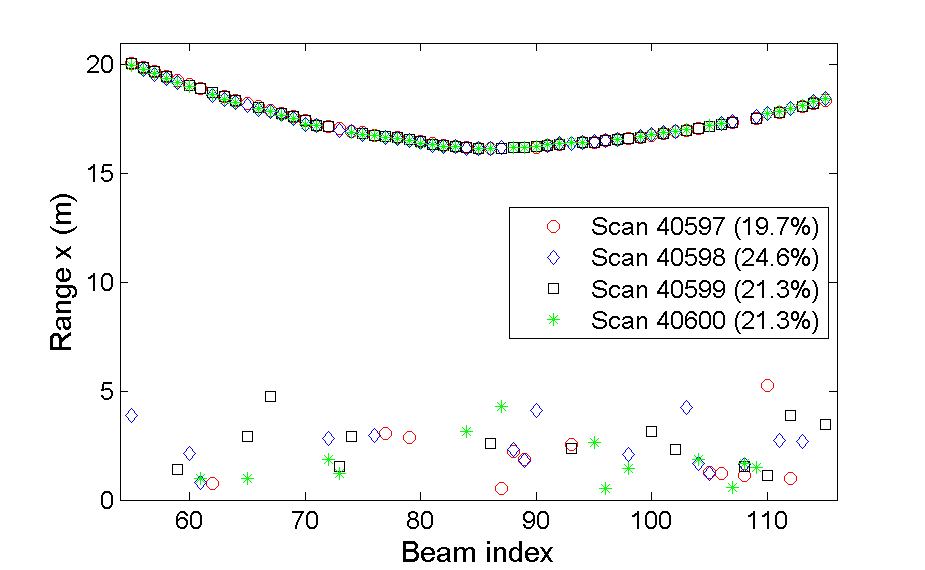
\includegraphics[width=0.95\linewidth]{./img/LMS200_4Scans_Feb19.png}
    \caption{Four overlaid consecutive scans for the LMS200 sensor, taken in the 02-19 dataset. Each symbol correspond to a particular scan. The curved line at the top correspond to the snow surface on the ground. One can see the rapid variation of the snowflake echoes between scans, and how they are mostly limited to a range $x<$\SI{5}{\meter} .}
    \label{fig:LMS200_4Scans_Feb19}
\end{figure}


A significant side benefit of those more sensitive sensors is that hey are able to record the timeline of a snow storm at a temporally fine-grained. This is something that is not possible with traditional snow measuring equipment, which can only report accumulation over long period of times. Indeed, for b) we see a pretty steady snowfall from t=1 to t=4 hours, with a peak around t=1.25 hours. This could be helpful in modeling a snowstorm in a simulator. 



For the Hokuyo, we plot two data: 1st and last echo. We do this o allow for fair comparison, as this device is, by design, returning echos in the falling snow. Moreover, it allows us to have an idea of how much  snow is actually falling. Note that however there was instance (daytime with sun) where the sensor didn't return  echos at all. We suspect that this is sue to the fact that the power level used

\begin{figure*}[th]
    \centering
    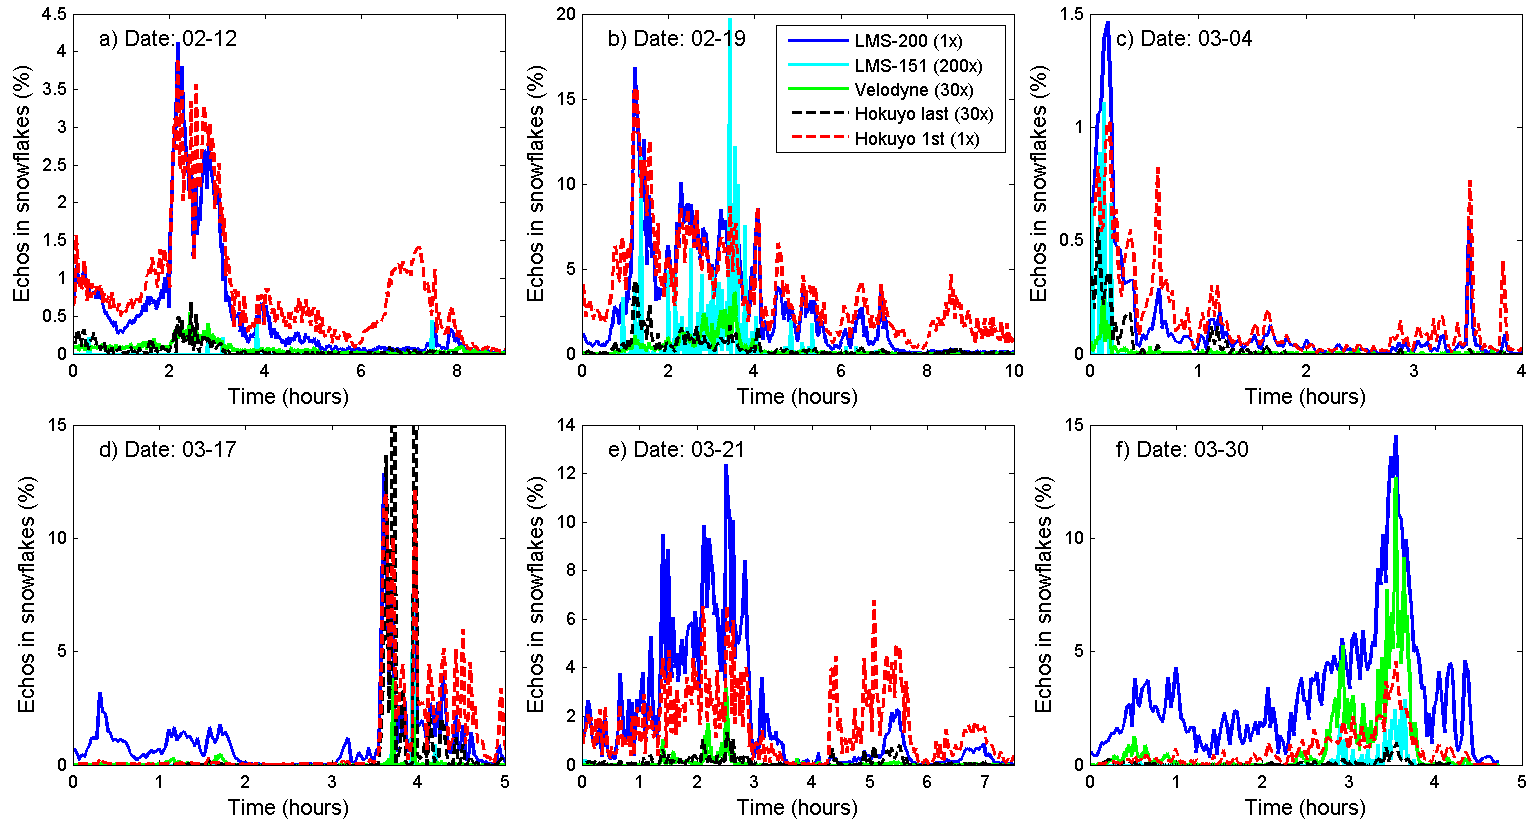
\includegraphics[width=0.98\linewidth]{./img/TimingSnow.png}
    \caption{Timing for snow. More to come.}
    \label{fig:TimingSnow}
\end{figure*}


% ========================= Histograms ===================
\subsection{Distribution of Echos in Falling Snowflakes, as a function of distance}
\label{subsub:Histo}

Fig. \ref{fig:Histograms} shows the histogram distribution of the snowflake echoes, as a function of distance. In some ways, they give us an approximate probability density function of these echoes that could be used to model such sensors. To allow for ease of comparison, these histograms have all been normalized by their total area. The numbers in brackets in the legend indicate the fraction of echoes in the snowflakes, compared to the total number of data points. The general shape (for the most part) of these histograms is close to a log-normal distribution, with the exception of the LMS200 for a number of dates (02-12 through 03-17), which seems to follow a sum of log-normal distributions. This indicate that a simple probabilistic model can be derived for these sensors.
%, such as
%\begin{equation}
%p(e|x,w)=p(e|w)p(e|x)
%\end{equation}
%where p(e|x) would be the log-normal distribution and p(e|w) the probability of having snow affecting

These histograms can be broken down into two main regions of interest. The first half (located from the left hand side of the peak) shows an exponential increase in snowflake echoes as a function of the distance x. We attribute this phenomenon to the shielding effect of the building from the falling snow. This phenomenon would be more or less absent on an autonomous vehicle, and thus we do not consider it much in our analysis. At the peak, this shielding effect effectively vanishes. The right hand side of the peak shows a gaussian-type exponential decrease of the probability of echos in falling snow. This could be explained by the greatly reduced light intensity (1/$x^2$) of the return, coupled with the decreased light flux/intensity if one assume constant beam size on the way out. This is great news, 

For the LMS151, the amound of data is not sufficient to draw much conclusion on this distribution except for the fact that there was virtually no events passed 4.


\begin{figure}[th]
    \centering
    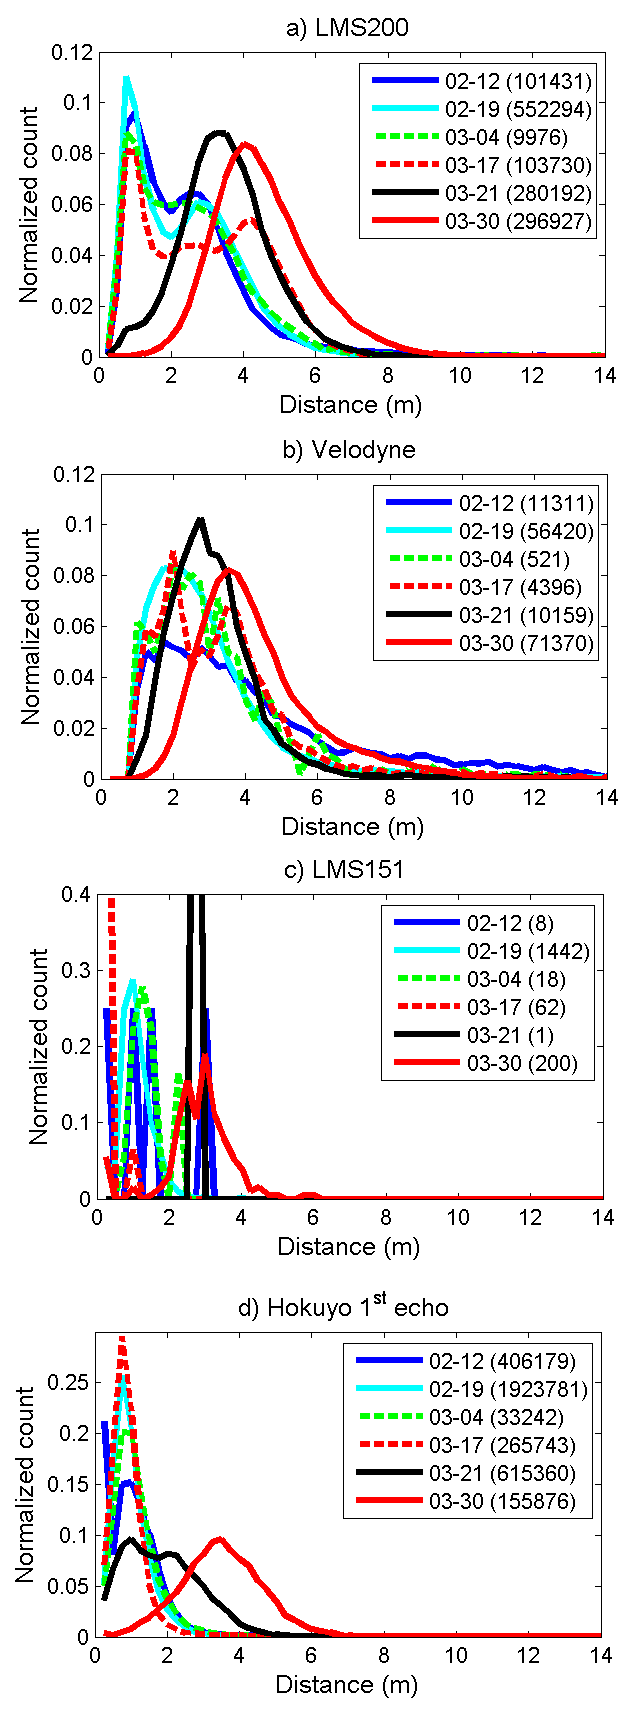
\includegraphics[width=0.80\linewidth]{./img/Histograms.png}
    \caption{Histograms of echoes in falling snow during important snowfall days, as a function of distance $x$ reported by the sensor. Each histogram has been normalized by its area, for ease of comparison. The numbers in brackets are the fraction of data points in the complete data set that correspond to snowflake echoes. Note that for the 03-21 dataset, the LMS151 was not working properly: thus no data is included for that day.}
    \label{fig:Histograms}
\end{figure}

Results show that laser might need to be mounted farther away from the front of the car, so as to avoid the first 1-2 meters that contain significant amount of echos. Or adjust threshold as a function of speed.

% ======================= Sunlight =====================
\subsection{Impact of sunlight on Hokuyo}
